% =============================================================================
%  Dinamica3_Fase3_Diapositiva1.tex — Dinámica 3, Fase 3, Diapositiva 1:
%  lectura con tensión. Texto en español limpio (el resumen de la Fase 2)
%  mientras el audio comienza a volverse molesto: el pergamino se oscurece en
%  los bordes y aparecen las primeras luces saturadas.
%  Formato 16:9. Compilar con: bash ../../../compilar_diapositivas.sh
% =============================================================================
\documentclass[tikz,border=0pt]{standalone}
\usepackage[utf8]{inputenc}
\usepackage[T1]{fontenc}
\usepackage{ebgaramond}
\usetikzlibrary{fadings}
\frenchspacing
\hyphenpenalty=10000 \exhyphenpenalty=10000   % sin división de palabras

% ── Parámetros ────────────────────────────────────────────────────────────────
\def\TamLetra{30}       % tamaño de letra, en pt
\def\Interlinea{42}     % interlineado, en pt
\def\AnchoTexto{25}     % ancho del bloque de texto, en cm
\def\NumLuces{14}       % luces saturadas en los bordes

% ── Paleta ────────────────────────────────────────────────────────────────────
\definecolor{Pergamino}{HTML}{F1EBDD}
\definecolor{PergaminoTension}{HTML}{C9A877}   % borde más oscuro y saturado
\definecolor{Fibra}{HTML}{B9A27A}
\definecolor{Tinta}{HTML}{2B2620}
\definecolor{Etiqueta}{HTML}{6B3E12}
\definecolor{Referencia}{HTML}{5E4C35}
\definecolor{LuzNaranja}{HTML}{FF6B1A}
\definecolor{LuzMagenta}{HTML}{E8368F}
\definecolor{LuzCian}{HTML}{22B8CF}
\definecolor{LuzAmarilla}{HTML}{FFD23F}

% ── Dimensiones (16:9) ────────────────────────────────────────────────────────
\def\ancho{32}
\def\alto{18}

\begin{document}
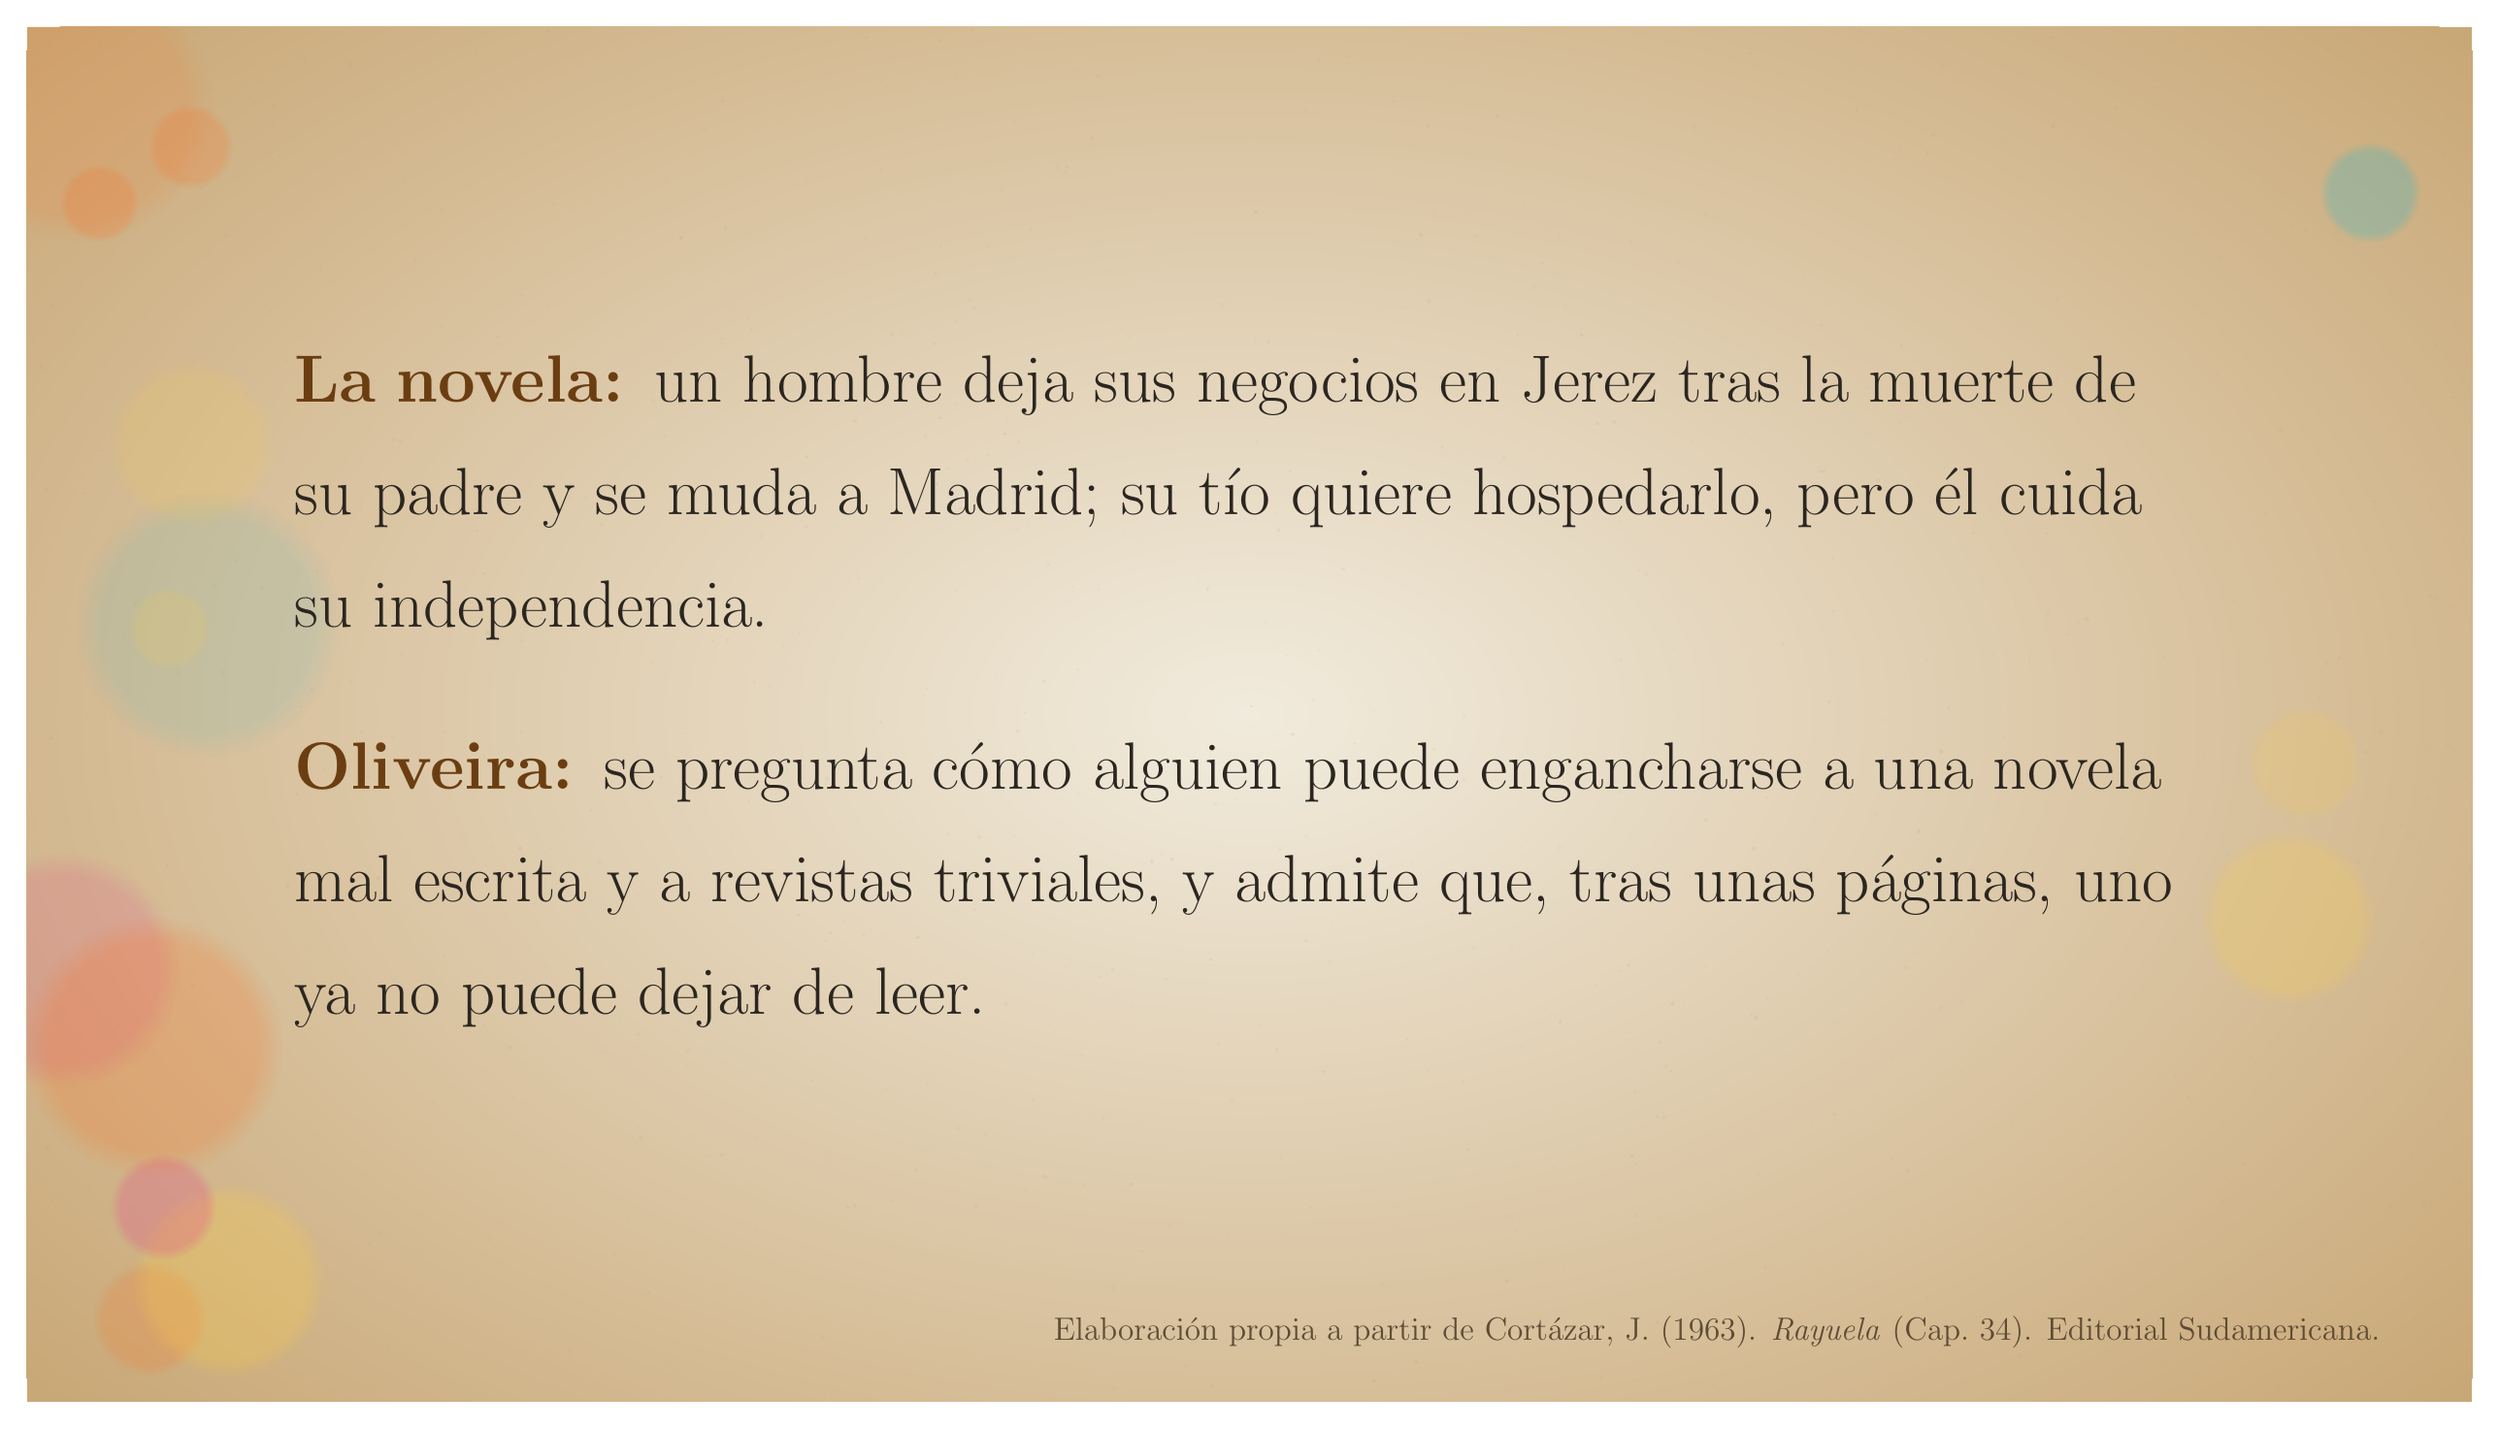
\begin{tikzpicture}
  \useasboundingbox (0,0) rectangle (\ancho,\alto);
  \clip (0,0) rectangle (\ancho,\alto);

  % Fondo: viñeta más marcada que en las fases anteriores
  \fill[PergaminoTension] (0,0) rectangle (\ancho,\alto);
  \shade[inner color=Pergamino, outer color=PergaminoTension]
    (\ancho/2,\alto/2) ellipse [x radius=0.66*\ancho, y radius=0.74*\alto];

  % Textura (misma semilla que la Fase 1)
  \pgfmathsetseed{1914}
  \foreach \i in {1,...,900}{
    \pgfmathsetmacro{\x}{rnd*\ancho}
    \pgfmathsetmacro{\y}{rnd*\alto}
    \pgfmathsetmacro{\r}{0.008+0.02*rnd}
    \pgfmathsetmacro{\o}{0.05+0.12*rnd}
    \fill[Fibra, opacity=\o] (\x,\y) circle (\r);
  }

  % Primeras luces saturadas, solo en las orillas (fuera del bloque de texto)
  \pgfmathsetseed{68}
  \foreach \i in {1,...,\NumLuces}{
    \pgfmathsetmacro{\lado}{rnd}
    \pgfmathsetmacro{\x}{\lado<0.5 ? 0.3+2.6*rnd : \ancho-0.3-2.6*rnd}
    \pgfmathsetmacro{\y}{rnd*\alto}
    \pgfmathsetmacro{\r}{0.5+1.3*rnd}
    \pgfmathsetmacro{\o}{0.10+0.15*rnd}
    \pgfmathtruncatemacro{\c}{int(4*rnd)}
    \ifcase\c\relax \def\col{LuzNaranja}\or \def\col{LuzMagenta}%
      \or \def\col{LuzCian}\else \def\col{LuzAmarilla}\fi
    \fill[\col, fill opacity=\o, path fading=circle with fuzzy edge 20 percent]
      (\x,\y) circle (\r);
  }

  % Texto limpio
  \node[text=Tinta, align=left, text width=\AnchoTexto cm, inner sep=0pt,
        font=\fontsize{\TamLetra}{\Interlinea}\selectfont]
    at (\ancho/2,\alto/2+0.3) {%
      {\color{Etiqueta}\bfseries La novela:} un hombre deja sus negocios en
      Jerez tras la muerte de su padre y se muda a Madrid; su tío quiere
      hospedarlo, pero él cuida su independencia.\par\vspace{0.8em}
      {\color{Etiqueta}\bfseries Oliveira:} se pregunta cómo alguien puede
      engancharse a una novela mal escrita y a revistas triviales, y admite
      que, tras unas páginas, uno ya no puede dejar de leer.%
    };

  % Referencia
  \node[anchor=south east, text=Referencia, inner sep=0pt,
        font=\fontsize{13}{16}\selectfont]
    at (\ancho-1.2,0.7)
    {Elaboración propia a partir de Cortázar, J. (1963). \textit{Rayuela} (Cap.~34). Editorial Sudamericana.};
\end{tikzpicture}
\end{document}
